% \documentclass{beamer}
\documentclass[14pt,mathserif]{beamer}


% \usepackage[no-math]{fontspec}

% \usepackage{xunicode,xltxtra} 
% \setmonofont[Scale=MatchLowercase,Numbers=Monospaced]{Andale Mono}
% \defaultfontfeatures{Numbers=OldStyle}
% \defaultfontfeatures{Ligatures=NoCommon}
% \setsansfont[BoldFont=Myriad Pro Semibold]{Myriad Pro}

% \usepackage{wrapfig}
\usepackage{hyperref}
\usepackage{textpos}
\usepackage{subcaption}

\usepackage{nicefrac}
% \usepackage{beamerthemesplit} // Activate for custom appearance
\setbeamertemplate{footline}[frame number]
\beamertemplatenavigationsymbolsempty

%\setbeamercovered{transparent}
%\usetheme{Pittsburgh}
%\usetheme{Rochester}

\useinnertheme{circles}

\usepackage{upquote}

\newcommand{\laquo}{“}
\newcommand{\raquo}{”}
\newcommand{\apos}{‘}

\setbeamertemplate{blocks}[rounded][shadow=true]

% \setbeamertemplate{frametitle}[default][center]
\setbeamertemplate{frametitle}
{
  \begin{centering}
    \textbf{\insertframetitle}
    \par
  \end{centering}
  \vspace{-1mm}
}
\setbeamertemplate{background}{
\includegraphics[width=\paperwidth]{slide_bg.png}} 
\definecolor{coolblue}{RGB}{0,88,100}
\definecolor{darkerred}{RGB}{207,83,0}
\definecolor{coolblue2}{RGB}{0,72,87}
\definecolor{lightgr}{RGB}{240,240,240}

\setbeamercolor{structure}{fg=coolblue}
\setbeamercolor{alerted text}{fg=darkerred}
\setbeamercolor{normal text}{fg=coolblue2}
\setbeamercolor{block title}{fg=coolblue, bg=lightgr}

\title{\huge \textbf{Deep Learning for the Real World}}
\subtitle{Annuli Detection in ultrasound images}
\author{Marcel~Ruegenberg \and Anupama~Jha \and Sandip~Mukherjee}
\date{July 24, 2013}

\begin{document}
%
%\frame{
%\titlepage
%}

\begin{frame}
\maketitle
\begin{textblock*}{1.731cm}(9.7cm,-0.5cm)
  
\includegraphics[width=1.53cm]{tumlogo2.png}
\end{textblock*}
\begin{textblock*}{2cm}(-0.5cm,-0.7cm)
  
\includegraphics[width=1cm]{inlogo.png}
\end{textblock*}

\end{frame}


% \begin{frame}
% \centering
% \huge{\textbf{Algorithmic\\Mechanism Design}}\\
% \large{Noam Nisan, Amir Ronen}\\\ \\
% \small 2001
% \begin{textblock*}{1.731cm}(9.6cm,1.8cm)
%   
\includegraphics[width=1.53cm]{tumlogo2.png}
% \end{textblock*}
% \begin{textblock*}{2cm}(-1.0cm,1.6cm)
%   \includegraphics[width=1cm]{inlogo2.png}% use the \includegraphics command here
% \end{textblock*}

% \end{frame}

\AtBeginSection{
\begin{frame}
\begin{center}
\structure{\LARGE \textbf{\insertsection}}
\end{center}
\end{frame}
}


% \frame{
% \frametitle{Outline}
% \tableofcontents
% }

\section{Dataset \& Task}

\begin{frame}

  \begin{itemize}
     \setlength{\itemsep}{1em}
      \item In ultrasound of the heart, detect annuli
        \\(rings around the heart valves)
      \item<1-> Examples:\\
        \begin{figure}
           \begin{subfigure}{0.28\textwidth}
             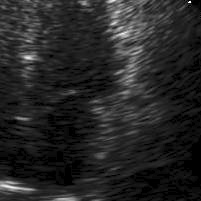
\includegraphics[width=\textwidth]{examples/1077_4ch_r.jpg}
           \end{subfigure}
           \begin{subfigure}{0.28\textwidth}
             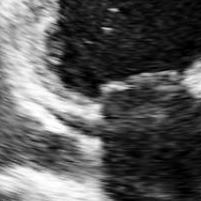
\includegraphics[width=\textwidth]{examples/3444_2ch_l.jpg}
           \end{subfigure}
           \begin{subfigure}{0.28\textwidth}
             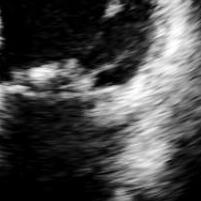
\includegraphics[width=\textwidth]{examples/3558_4ch_r.jpg}
           \end{subfigure}
        \end{figure}
      \item<1-> Annulus roughly at the center of each sample
      \end{itemize}
 \end{frame}


\subsection{Preprocessing \& Building the Dataset}

\frame
{
  \frametitle{Preprocessing}

  \setlength{\leftmargini}{0em}
  \setlength{\leftmarginii}{1em}
  \begin{itemize}
     \setlength{\itemsep}{1em}
      \item Images contained artefacts:
        \begin{itemize}
        \item Scales
        \item Lines from ultrasound device
      \only<1-1>{
      \begin{figure}
           \begin{subfigure}{0.28\textwidth}
             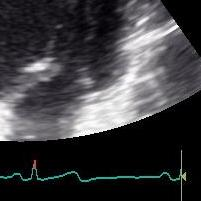
\includegraphics[width=\textwidth]{examples/0515_4ch_r.jpg}
           \end{subfigure}
           \begin{subfigure}{0.28\textwidth}
             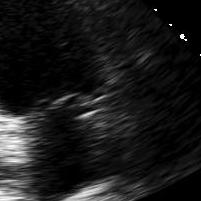
\includegraphics[width=\textwidth]{examples/0599_2ch_r.jpg}
           \end{subfigure}
           \begin{subfigure}{0.28\textwidth}
             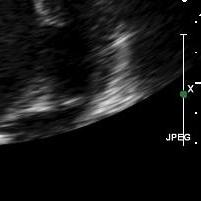
\includegraphics[width=\textwidth]{examples/0627_2ch_r.jpg}
           \end{subfigure}
        \end{figure}
        }
        \only<2->{
      \begin{figure}
           \begin{subfigure}{0.28\textwidth}
             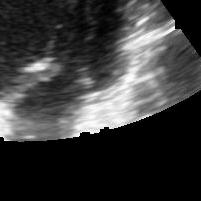
\includegraphics[width=\textwidth]{examples/cleaned/0515_4ch_r.jpg}
           \end{subfigure}
           \begin{subfigure}{0.28\textwidth}
             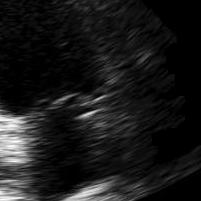
\includegraphics[width=\textwidth]{examples/cleaned/0599_2ch_r.jpg}
           \end{subfigure}
           \begin{subfigure}{0.28\textwidth}
             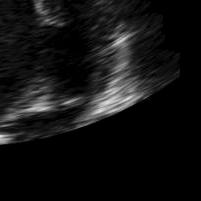
\includegraphics[width=\textwidth]{examples/cleaned/0627_2ch_r.jpg}
           \end{subfigure}
        \end{figure}
        }
      \item Fixed by masking colored/purely white pixels; 
        flood~fill; image morphology operations (dilation / erosion)
      \end{itemize}
    \item<3-> Standard data normalization: $\tilde{X} = \frac{X - \mu}{\sigma}$
    \setlength{\leftmargini}{2em}
  \end{itemize}
}

\frame
{
  \frametitle{Building the dataset}

  \setlength{\leftmargini}{0em}
  \setlength{\leftmarginii}{1em}
  \begin{itemize}
     \setlength{\itemsep}{1em}
      \item Dataset only has 2 classes: \emph{left} and \emph{right} annulus
      \item Training requires 3rd class: \emph{no annulus}
        \begin{itemize}
          \item<2-> Build the dataset from smaller patches in the image
            ($20 \times 20 \text{px}$ or $60 \times 60 \text{px}$).
          \item<2-> Take center patches of
            images as annulus, take surrounding patches as ``no annulus''.
          \item<3-> Shuffle found patches, then split into
            training/set/validation set (60/20/20).
          \end{itemize}
          \setlength{\leftmargini}{2em}
  \end{itemize}
}

\frame
{
  \frametitle{First approaches}
  \begin{itemize}
     \setlength{\itemsep}{1em}
     \item Standard  Feed forward Neural Network
      \begin{itemize}
      	\item 1 Hidden layer, 0.1 learning rate 					and rmsprop	
        	\item Best result obtained : 17\%
        	\end{itemize}
   \end{itemize}
   \begin{itemize}
     \setlength{\itemsep}{1em}
     \item Plots for 2ch 60x60 patch with 2 class 
     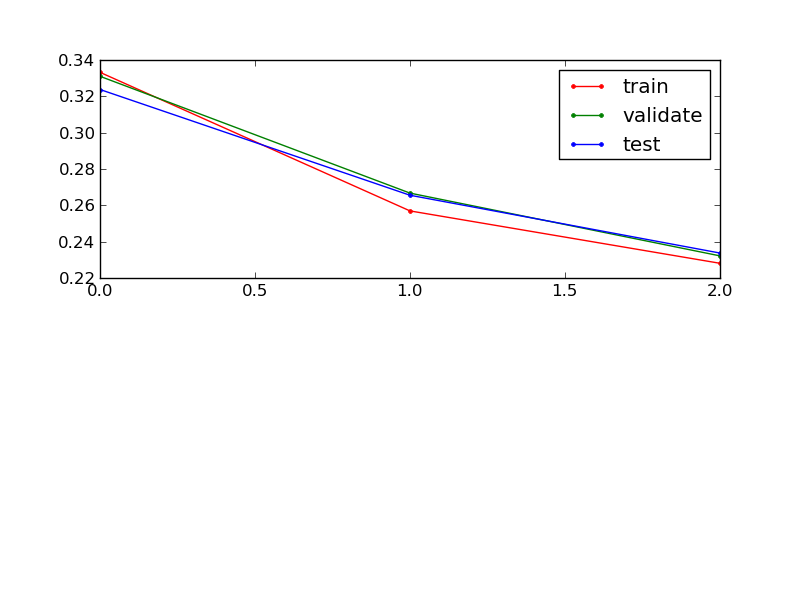
\includegraphics[scale=0.35]{standard_NN_2class_errors.png}     	
  	\end{itemize}
}

\frame
{
  \frametitle{Standard NN with Dropout}
  \begin{itemize}
     \setlength{\itemsep}{1em}
     \item Implementation Details
      \begin{itemize}
      	\item 1 Hidden layer, with 1200 neurons size
        	\item 50\% dropout on hidden layers,20\% dropout on input layer
        	\item Used theano.binomial to create the mask with given probability
        	\item Momentum and weight updation is done according to Hinton's paper
        	\item decay of learning rate after each epoch
        	\end{itemize}
   \end{itemize}
   \begin{itemize}
     \setlength{\itemsep}{1em}
     \item Challenges
     	\begin{itemize}
     	\item Determination of maximum squared length limit for incoming weights
     	\item Number and dimension of hidden layers
     	\item High dimension for hidden layers like 4200 didn't work so well
     	\end{itemize}
  	\end{itemize}
}

\frame
{
  \frametitle{Result with NN Dropout}
  \begin{itemize}
     \setlength{\itemsep}{1em}
     \item Performance improved from standard NN
      \begin{itemize}
      	\item 4\% test error for 2class unbalanced set
        	\item 6\% error for multiclass unbalanced test set
        	\end{itemize}
   \end{itemize}
   \begin{itemize}
     \setlength{\itemsep}{1em}
     \item Plots for 2ch 60x60 patch with 2 class   	
  	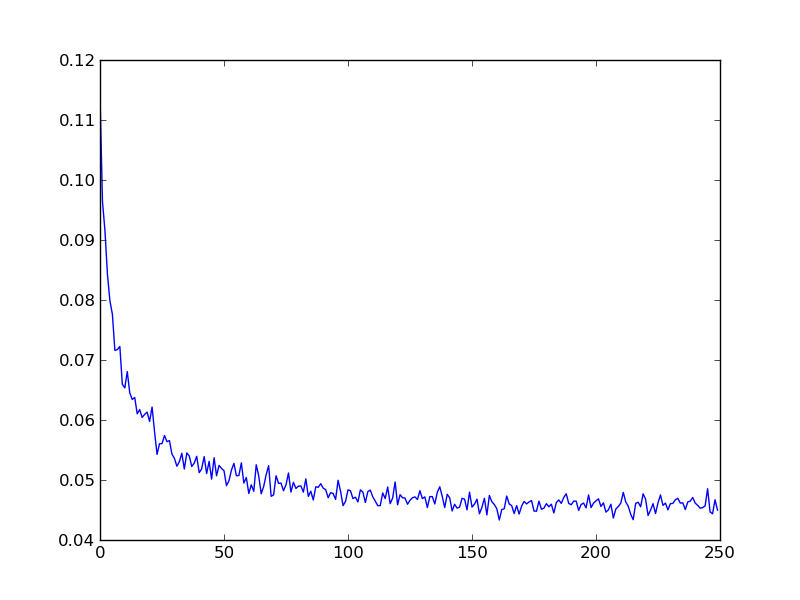
\includegraphics[scale=0.35]{NN_dropout_2class_validation_error.png} 
  	\end{itemize}
}

\frame
{
  \frametitle{Dropout Result(Contiued)}
  \begin{itemize}
     \setlength{\itemsep}{1em}
     \item Plots of 2ch 60x60 patch multiclass
     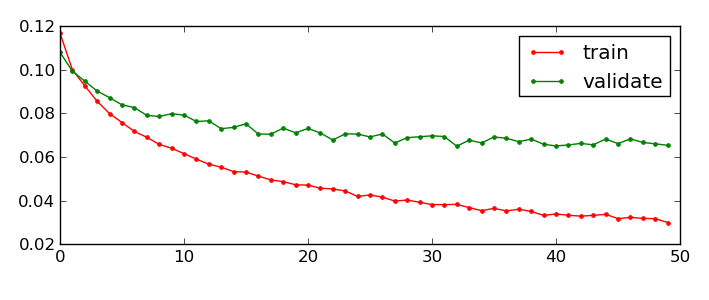
\includegraphics[scale=0.50]{3class_errors.png}  
   \end{itemize}
   \begin{itemize}
     \setlength{\itemsep}{1em}
     \item Future Scope
     \begin{itemize}
     	\item Pre-trained DBN with dropout
     	\item Dropout on last hidden layer of Convolutional Neural Network
     \end{itemize}
  	\end{itemize}
}


\frame
{
  \frametitle{Convolutional Neural Network}

  \setlength{\leftmargini}{0em}
  \setlength{\leftmarginii}{1em}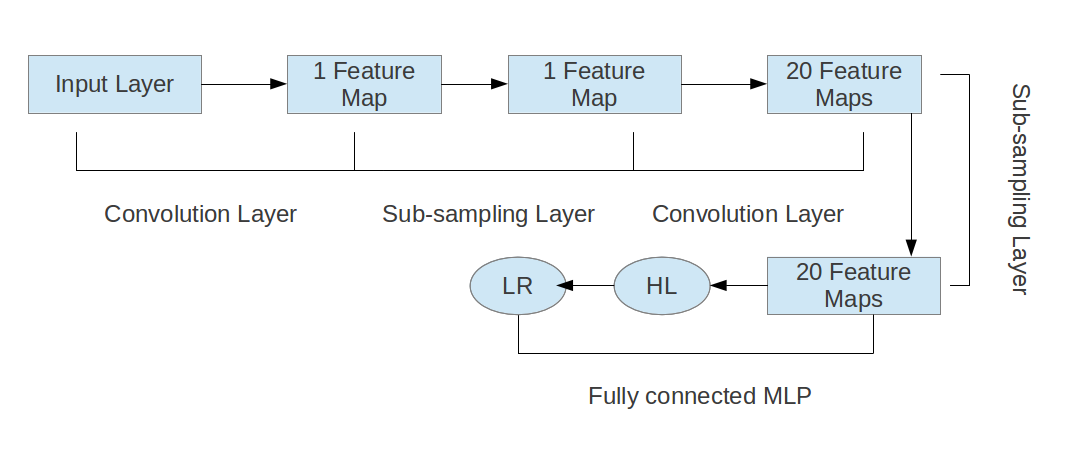
\includegraphics[scale=0.3]{cnn.png} 
}

\frame
{
  \frametitle{CNN: Details}

  \setlength{\leftmargini}{0em}
  \setlength{\leftmarginii}{1em}
   \begin{itemize}
     \setlength{\itemsep}{1em}
     \item Convolutional Layer 1
      \begin{itemize}
      	\item 20 Filters of 5 x 5
        	\item Maxpooling by the factor (2, 2)
        	\end{itemize}
      \item Convolutional Layer 2
      	\begin{itemize}
      	\item 50 Filters of 5 x 5
        	\item Maxpooling by the factor (2, 2)
        	\end{itemize}
     \item Hidden Layer
      \begin{itemize}
      	\item Input: (number of Filters of CL2) * (CL2 output size)${^{2}}$
        	\item Output: 500 
        	\end{itemize}
   \end{itemize}
}

\frame
{
  \frametitle{CNN: Details}

  \setlength{\leftmargini}{0em}
  \setlength{\leftmarginii}{1em}
   \begin{itemize}
     \setlength{\itemsep}{1em}
      \item Logistic Regression Layer
      	\begin{itemize}
      	\item Input: 500
        	\item Output: \\2 (Annuli or not) or 3 (left, right or no Annuli) classes 
        	\end{itemize}
      \item Hyperparameters: Minibatch Gradient Descent
      	\begin{itemize}
      	\item Learning Rate: 0.1
      	\item Epochs: 20
        	\end{itemize}
   \end{itemize}
  
}
\frame
{
  \frametitle{Additional tricks}
	\begin{itemize}
	\item Convolutional Neural Network with rmsprop and Momentum \\
         Hyperparameters: RMSPROP
      	\begin{itemize}
      	\item Learning Rate: 0.0001
        	\item Momentum: 0.7 
        	\end{itemize}
     \item Neural Network with dropout
   \end{itemize}
  % 
}

\frame
{
  \frametitle{Results: CNN-MSGD}
	2 chamber Images, 20 x 20 patches  
  	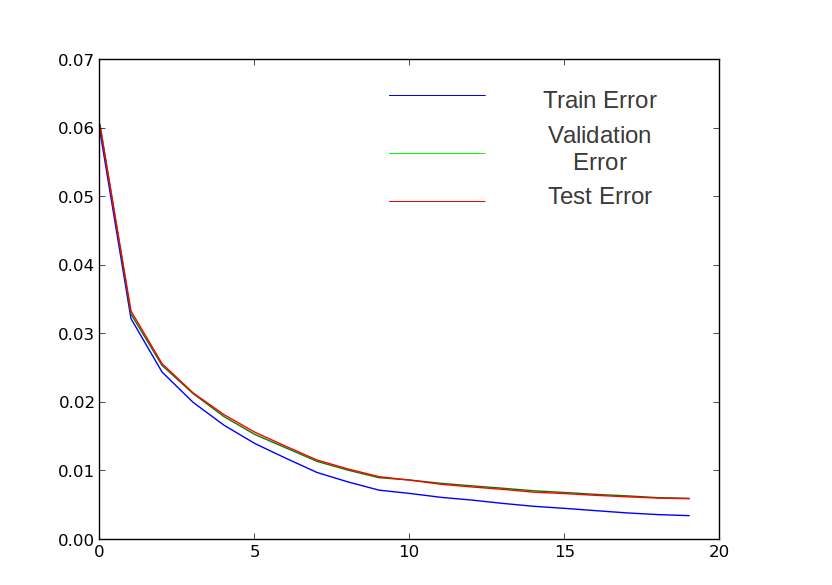
\includegraphics[scale=0.35]{errorcnn2ch20px.png} 
}

\frame
{
  \frametitle{Results: CNN-MSGD}
	Best validation Error: 0.606816 \% \\
	Best Test Error: 0.602769 \% \\
	Train, validation and test data was balanced, but results were not much different then unbalanced test set \\
	True Positive(Annuli) 49.9218 \% \\ 
	True Negative(Non Annuli) 49.4754 \% \\
	False Positive 0.5798 \% \\
	False Negative 0.0230 \% \\
}


\frame
{
  \frametitle{Result and Classifier}
 \begin{itemize}
     \setlength{\itemsep}{1em}
     \item Plots of 2ch 60x60 patch with CNN rmsprop
     \begin{itemize}
     	\item Validation Error: 0.676190 \%
		\item Test Error: 0.600000 \%
     \end{itemize}
     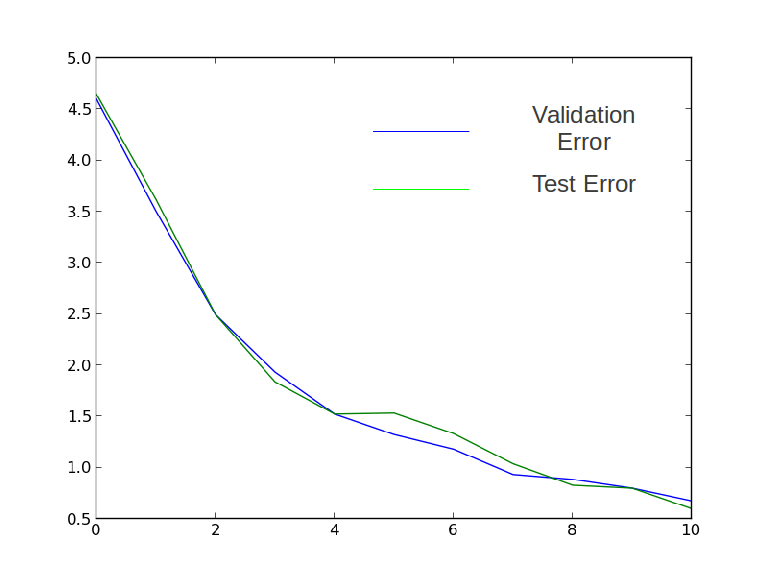
\includegraphics[scale=0.15]{error_testCNN_rmsprop.png}  
   \end{itemize}
   \begin{itemize}
     \setlength{\itemsep}{1em}
     \item Classifier
     \begin{itemize}
     	\item It takes directory of images
     	\item Do all the preprocessing and create patches from images
     	\item Use previosuly saved weights
     	\item And finally predict whether the image has annulli or not
     \end{itemize}
  	\end{itemize}
}


\frame
{
\begin{center}
\Huge Questions?\\\ \\\ \\
\normalsize

\end{center}
}

\frame
{
\begin{center}
 \Huge Thank you
\end{center}
}


\end{document}
